\documentclass[10pt, aspectratio=169, handout]{beamer}
\usefonttheme{professionalfonts}

\mode<presentation>{
  \usetheme{Berkeley}
  \usecolortheme{beaver}
  \usefonttheme{default}
  \setbeamertemplate{navigation symbols}{}
  \setbeamertemplate{caption}[numbered]
}

\setbeamertemplate{footline}{%
  \leavevmode%
  \hbox{%
    \begin{beamercolorbox}[wd=.85\paperwidth,ht=2.5ex,dp=1ex,left]{author in head/foot}%
      \usebeamerfont{author in head/foot}Digital Signal Processing, Fall 2025%
    \end{beamercolorbox}%
    \begin{beamercolorbox}[wd=.15\paperwidth,ht=2.5ex,dp=1ex,right]{date in head/foot}%
      \hspace*{0.5em}\insertframenumber{} / \inserttotalframenumber\hspace*{0.5em}%
    \end{beamercolorbox}%
  }%
  \vskip0pt%
}

\usepackage[english]{babel}
\usepackage[utf8]{inputenc}
\usepackage{tikz}
\usepackage{pgfplots}
\usepgfplotslibrary{groupplots}
\usetikzlibrary{calc, positioning, arrows.meta, backgrounds, pgfplots.groupplots, plotmarks}
\pgfplotsset{compat=newest}

\usepackage{array}
\usepackage{makecell}
\usepackage{verbatim}
\usepackage{graphicx}
\usepackage{amsfonts}
\usepackage{amsmath}
\usepackage{bm}
\usepackage{epstopdf}
\usepackage[absolute,overlay]{textpos}
\usepackage{hyperref}
\hypersetup{colorlinks=true, linkcolor=blue, urlcolor=cyan}

\title[ECEN 463/863]{Sampling Rate Conversions: Upsampling (Interpolation)}
\author{Maxx Seminario}
\institute{University of Nebraska-Lincoln}
\date{Fall 2025}

\begin{document}

%--------------------------------------------------
\begin{frame}
  \titlepage
\end{frame}

%--------------------------------------------------
\section{Motivation and Definitions}

\begin{frame}{Motivation for Upsampling}
\small
\textbf{Why increase the sampling rate?}
\begin{itemize}
  \item Interface between systems running at different sample rates (audio, telecom, sensors).
  \item Enable finer time resolution for subsequent processing (filtering, D/A conversion).
\end{itemize}

\vspace{0.4cm}
\textbf{Goal:} Given samples \(x[n] = x_c(nT)\), produce samples
\[
x_i[n] = x_c(nT_i), \qquad T_i = \frac{T}{L}
\]
so that the new sampling rate is \(L\) times larger.


\end{frame}

\begin{frame}{Upsampling: Definition and Approach}
\small

\textbf{Definition (Upsampling / Interpolation):}
\[
x_i[n] = x\!\left[\frac{n}{L}\right] = x_c\!\left(\frac{nT}{L}\right), \quad n = 0, \pm L, \pm 2L, \dots
\]

At integer multiples of \(L\), we have the original samples. Elsewhere, we need intermediate values.

\vspace{0.4cm}
\textbf{Problem:} Need the ``missing'' samples while preserving bandlimited structure.

\vspace{0.4cm}
\textbf{Solution Outline:}
\begin{enumerate}
  \item \textbf{Expand:} Insert \(L-1\) 'null' samples between each original sample (creates \(x_e[n]\)).
  \item \textbf{Interpolate:} Lowpass filter with gain \(L\) and cutoff \(\pi/L\) to reconstruct intermediate samples.
\end{enumerate}

\vspace{0.2cm}
This process preserves the bandlimited nature of the signal.

\end{frame}

%--------------------------------------------------
\begin{frame}{Expander and Interpolator Structure}
\small
\textbf{Expander (Sampling Rate Expander):}
\[
x_e[n] = \begin{cases}
x[n/L], & n = 0, \pm L, \pm 2L, \dots \\
0, & \text{otherwise}
\end{cases}
\quad \Longleftrightarrow \quad x_e[n] = \displaystyle \sum_{k=-\infty}^{\infty} x[k]\, \delta[n - kL]
\]

\textbf{Interpolator:} Lowpass filter \(h_i[n]\) (gain \(L\), cutoff \(\pi/L\)) applied to \(x_e[n]\):
\[
x_i[n] = (h_i * x_e)[n]
\]

\vspace{0.3cm}
\textbf{System Diagram:}
\begin{center}
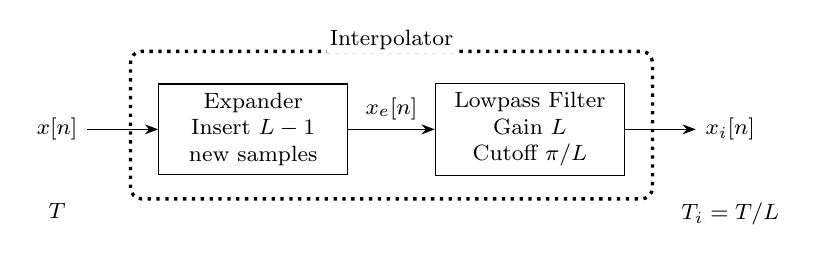
\begin{tikzpicture}[>=Stealth, node distance=0.9cm, every node/.style={font=\footnotesize}]
  \tikzset{block/.style={draw, minimum width=2.4cm, minimum height=1.0cm, align=center}}
  \node (xn) {$x[n]$};
  \node[block, right=0.9cm of xn] (expand) {Expander\\Insert $L-1$ \\ new samples};
  \node[block, right=1.1cm of expand] (lpf) {Lowpass Filter\\Gain $L$\\Cutoff $\pi/L$};
  \node (xin) [right=0.9cm of lpf] {$x_i[n]$};

  \draw[->] (xn.east) -- (expand.west);
  \draw[->] (expand.east) -- node[midway, above] {$x_e[n]$} (lpf.west);
  \draw[->] (lpf.east) -- (xin.west);

  \node[below=0.55cm of xn] {$T$};
  \node[below=0.55cm of xin] {$T_i = T/L$};

  % Dotted outline around the interpolator (Expander + Lowpass Filter)
  \coordinate (boxSW) at ($(expand.south west)+(-0.35,-0.30)$);
  \coordinate (boxNE) at ($(lpf.north east)+(0.35,0.40)$);
  \draw[dotted, very thick, rounded corners] (boxSW) rectangle (boxNE);

  % Label ABOVE the dotted outline (top-center)
  \path let \p1=(boxSW), \p2=(boxNE) in coordinate (boxTopCenter) at ({(\x1+\x2)/2}, {\y2});
  \node[font=\footnotesize, fill=white, inner sep=1pt] at ([yshift=4pt]boxTopCenter) {Interpolator};
\end{tikzpicture}
\end{center}

\textbf{Terminology:} Expander + Antialias (Interpolation) Filter = \textbf{Interpolator}.
\end{frame}

%--------------------------------------------------
\begin{frame}{Frequency-Domain Effect of Expansion: DTFT of $x_e[n]$}
\small
\textbf{Expander definition:}
\[
x_e[n] =
\begin{cases}
x[n/L], & n = 0, \pm L, \pm 2L, \dots \\
0, & \text{otherwise}
\end{cases}
\quad \Longleftrightarrow \quad
x_e[n] = \displaystyle \sum_{k=-\infty}^{\infty} x[k]\,\delta[n-kL]
\]

\textbf{Compute the DTFT of $x_e[n]$:}
\[
\begin{aligned}
X_e(e^{j\omega})
&= \sum_{n=-\infty}^{\infty} x_e[n]\; e^{-j\omega n} \\
&= \sum_{n=-\infty}^{\infty} \left(\sum_{k=-\infty}^{\infty} x[k]\,\delta[n-kL]\right) e^{-j\omega n} \\
&= \sum_{k=-\infty}^{\infty} x[k]\; e^{-j\omega (kL)} \\
&= \sum_{k=-\infty}^{\infty} x[k]\; e^{-j(\omega L) k} \\
&= X(e^{j\,\omega L})
\end{aligned}
\]

\textbf{Key result:}
\[
\boxed{\,X_e(e^{j\omega}) = X(e^{j\omega L})\,}
\]

\textbf{Immediate consequence:} The frequency variable is scaled by $L$ (i.e., the baseband spectrum appears compressed by $L$ in $X_e$).
\end{frame}

\begin{frame}{Frequency-Domain Effect of Expansion: Interpretation and Filter}
\small
\textbf{Result:}
\[
X_e(e^{j\omega}) = X(e^{j\omega L})
\]

\textbf{Interpretation:}
\begin{itemize}
  \item Baseband spectrum is \textbf{compressed} by factor $L$.
  \item Multiple frequency-scaled images appear within $|\omega|\le\pi$ due to DTFT periodicity.
  \item An interpolation lowpass (cutoff $\pi/L$) removes images and rescales amplitude.
\end{itemize}

\textbf{Interpolator output:}
\[
X_i(e^{j\omega}) = H_i(e^{j\omega})\,X_e(e^{j\omega}) \approx X(e^{j\omega}) \quad (\text{ideal})
\]

\textbf{Ideal interpolation filter:}
\[
H_i(e^{j\omega}) =
\begin{cases}
L, & |\omega|\le \pi/L \\
0, & \pi/L < |\omega|\le \pi
\end{cases}
\]

\textbf{Gain justification:} Scale by $L$ so spectral amplitude matches new sampling rate:
\[
L \cdot \frac{1}{T} \;=\; \frac{1}{T/L} \;=\; \frac{1}{T_i}.
\]
\end{frame}

% %--------------------------------------------------

\begin{frame}{Interpolation - Frequency Domain}
\small

\def\L{3} % <-- Set interpolation factor L here
% Precompute key angular points (in radians)
\pgfmathsetmacro{\piOverL}{pi/\L}
\pgfmathsetmacro{\twoPiOverL}{2*pi/\L}
\pgfmathsetmacro{\threePiOverL}{3*pi/\L}
\pgfmathsetmacro{\fourPiOverL}{4*pi/\L}
\pgfmathsetmacro{\fivePiOverL}{5*pi/\L}

\begin{center}
\begin{tikzpicture}[scale=0.8]
  \begin{groupplot}[
    group style={group size=1 by 4, vertical sep=1.1cm},  % Changed to 4 plots
    width=11.6cm,
    height=2.5cm,
    axis lines=middle,
    xmin=-11.1, xmax=11.1,
    ymin=0, ymax=1.15,
    tick label style={font=\scriptsize},
    label style={font=\scriptsize},
    title style={font=\scriptsize},
    xlabel={$\omega$}
  ]

  %------------------------------------------------------
  % Plot 1: Original spectrum
  %------------------------------------------------------
  \def\OmegaN{2.2}
  \nextgroupplot[
    title={$X_c(e^{j\omega})$ (Input Signal)},
    ytick={0,1},
    yticklabels={$0$,$1$},
    xtick={-10.9956,-9.4248,-7.85398,-6.2832,-4.7124,-3.1416,-1.5708,0,1.5708,3.1416,4.7124,6.2832,7.85398,9.4248,10.9956},
    xticklabels={$-7\pi/2$,$-3\pi$,$-5\pi/2$,$-2\pi$,$-3\pi/2$,$-\pi$,$-\pi/2$,$0$,$\pi/2$,$\pi$,$3\pi/2$,$2\pi$,$5\pi/2$,$3\pi$,$7\pi/2$}
  ]
  \addplot[blue!80!black, very thick] coordinates {
    (-11.1,0) (-\OmegaN,0) (0,1) (\OmegaN,0) (11.1,0)
  };
  \node[red!70!black, font=\scriptsize, anchor=north east] at (axis cs:-\OmegaN,0) {$-\Omega_N$};
  \node[red!70!black, font=\scriptsize, anchor=north west] at (axis cs:\OmegaN,0) {$+\Omega_N$};
  \node[blue!60!black, font=\scriptsize] at (axis cs:0,-0.23) {Bandwidth extends to $\pm\Omega_N$};

  %------------------------------------------------------
  % Plot 2: Three triangles centered at -2π, 0, 2π touching at ±π
  %------------------------------------------------------
  \nextgroupplot[
    title={$X(e^{j\omega})$ (Sampled Signal)},
    ytick={0,1},
    yticklabels={$0$,$1/T$},
    xtick={-9.4248,-6.2832,-3.1416,0,3.1416,6.2832,9.4248},
    xticklabels={$-3\pi$,$-2\pi$,$-\pi$,$0$,$\pi$,$2\pi$,$3\pi$}
  ]
  
  % Left triangle (center -2π)
  \addplot[green!60!black, thick, dotted]
    coordinates {
      (-9.4248,0) (-6.2832,1) (-3.1416,0)
    };
  % Center triangle (center 0)
  \addplot[blue!85!black, very thick]
    coordinates {
      (-3.1416,0) (0,1) (3.1416,0)
    };
  % Right triangle (center 2π)
  \addplot[orange!85!black, thick, dashed]
    coordinates {
      (3.1416,0) (6.2832,1) (9.4248,0)
    };

  % Vertical guide lines at touching edges
  \draw[gray!55,dotted] (axis cs:-9.4248,0) -- (axis cs:-9.4248,1.05);
  \draw[gray!55,dotted] (axis cs:-3.1416,0) -- (axis cs:-3.1416,1.05);
  \draw[gray!55,dotted] (axis cs:3.1416,0) -- (axis cs:3.1416,1.05);
  \draw[gray!55,dotted] (axis cs:9.4248,0) -- (axis cs:9.4248,1.05);

  \node[red!70!black, font=\scriptsize] at (axis cs:0,-0.25) {Replicas width $2\pi$ touch at $\pm\pi$};

  %------------------------------------------------------
  % Plot 3: Five touching triangles (k = -2,-1,0,1,2)
  %------------------------------------------------------
  \nextgroupplot[
    title={$X_e(e^{j\omega})$ (L = 2) (Post Expansion)},
    ytick={0,1},
    yticklabels={$0$,$1/T$},
    xtick={-5.2360,-3.1416,-1.0472,0,1.0472,3.1416,5.2360},
    xticklabels={$-5\pi/L$,$-3\pi/L$,$-\pi/L$,$0$,$\pi/L$,$3\pi/L$,$5\pi/L$}
  ]
  
  % k = -2 triangle (center -4π/L)
  \addplot[purple!70!black, thick, dashdotted]
    coordinates {
      (-\fivePiOverL,0) (-\fourPiOverL,1) (-\threePiOverL,0)
    };
  % k = -1 triangle (center -2π/L)
  \addplot[green!60!black, thick, dotted]
    coordinates {
      (-\threePiOverL,0) (-\twoPiOverL,1) (-\piOverL,0)
    };
  % k = 0 triangle (center 0)
  \addplot[blue!85!black, very thick]
    coordinates {
      (-\piOverL,0) (0,1) (\piOverL,0)
    };
  % k = 1 triangle (center 2π/L)
  \addplot[orange!85!black, thick, dashed]
    coordinates {
      (\piOverL,0) (\twoPiOverL,1) (\threePiOverL,0)
    };
  % k = 2 triangle (center 4π/L)
  \addplot[red!80!black, thick, dashdotdotted]
    coordinates {
      (\threePiOverL,0) (\fourPiOverL,1) (\fivePiOverL,0)
    };

  % Vertical guide lines at touching edges (explicit draws)
  \draw[gray!55,dotted] (axis cs:-\fivePiOverL,0) -- (axis cs:-\fivePiOverL,1.05);
  \draw[gray!55,dotted] (axis cs:-\threePiOverL,0) -- (axis cs:-\threePiOverL,1.05);
  \draw[gray!55,dotted] (axis cs:-\piOverL,0) -- (axis cs:-\piOverL,1.05);
  \draw[gray!55,dotted] (axis cs:\piOverL,0) -- (axis cs:\piOverL,1.05);
  \draw[gray!55,dotted] (axis cs:\threePiOverL,0) -- (axis cs:\threePiOverL,1.05);
  \draw[gray!55,dotted] (axis cs:\fivePiOverL,0) -- (axis cs:\fivePiOverL,1.05);

  \node[red!70!black, font=\scriptsize] at (axis cs:0,-0.25) {Replicas width $2\pi/L$ touch at odd multiples of $\pi/L$};

  %------------------------------------------------------
  % Plot 4: Three triangles 
  %------------------------------------------------------
  \nextgroupplot[
    title={$X_i(e^{j\omega})$ (Post LPF)},
    ytick={0,1},
    yticklabels={$0$,$L/T$},
    xtick={-5.2360,-3.1416,-1.0472,0,1.0472,3.1416,5.2360},
    xticklabels={$-5\pi/L$,$-3\pi/L$,$-\pi/L$,$0$,$\pi/L$,$3\pi/L$,$5\pi/L$}
  ]
  
  % k = -2 triangle (center -4π/L)
  \addplot[purple!70!black, thick, dashdotted]
    coordinates {
      (-\fivePiOverL,0) (-\fourPiOverL,1) (-\threePiOverL,0)
    };
  
  % k = 0 triangle (center 0)
  \addplot[blue!85!black, very thick]
    coordinates {
      (-\piOverL,0) (0,1) (\piOverL,0)
    };
  
  % k = 2 triangle (center 4π/L)
  \addplot[red!80!black, thick, dashdotdotted]
    coordinates {
      (\threePiOverL,0) (\fourPiOverL,1) (\fivePiOverL,0)
    };

  % Vertical guide lines at touching edges (explicit draws)
  \draw[gray!55,dotted] (axis cs:-\fivePiOverL,0) -- (axis cs:-\fivePiOverL,1.05);
  \draw[gray!55,dotted] (axis cs:-\threePiOverL,0) -- (axis cs:-\threePiOverL,1.05);
  \draw[gray!55,dotted] (axis cs:-\piOverL,0) -- (axis cs:-\piOverL,1.05);
  \draw[gray!55,dotted] (axis cs:\piOverL,0) -- (axis cs:\piOverL,1.05);
  \draw[gray!55,dotted] (axis cs:\threePiOverL,0) -- (axis cs:\threePiOverL,1.05);
  \draw[gray!55,dotted] (axis cs:\fivePiOverL,0) -- (axis cs:\fivePiOverL,1.05);

  \node[red!70!black, font=\scriptsize] at (axis cs:0,-0.25) {Three replicas (k = -2, 0, 2)};

  \end{groupplot}
\end{tikzpicture}
\end{center}

\end{frame}


%--------------------------------------------------
\section{Examples}

\begin{frame}{Example: Upsampling with $L=3$ }
\small
Assume original \(X(e^{j\omega})\) occupies \(|\omega| \le \pi/2\).

After expansion by \(L=3\):
\[
X_e(e^{j\omega}) = X(e^{j3\omega})
\]
Nonzero only for \(|\omega| \le \pi/6\) in principal lobe; other compressed images appear.

Interpolator \(H_i\):
\[
H_i(e^{j\omega}) = \begin{cases}
3, & |\omega| \le \pi/3 \\
0, & \pi/3 < |\omega| \le \pi
\end{cases}
\]

Result:
\[
X_i(e^{j\omega}) = H_i(e^{j\omega}) X_e(e^{j\omega}) \approx X(e^{j\omega})
\]

\textbf{Bandwidth Relation:} Needed cutoff \(\pi/3\) ensures only baseband compressed copy passes. Requires gain correction (Gain = 3).
\end{frame}

\begin{frame}{Example: $L=3$ (Frequency Domain Visualization)}
\small

\def\L{3} % Interpolation factor L = 3
% Precompute key angular points (in radians)
\pgfmathsetmacro{\piOverL}{pi/\L}        % π/3 = 1.0472
\pgfmathsetmacro{\twoPiOverL}{2*pi/\L}   % 2π/3 = 2.0944
\pgfmathsetmacro{\threePiOverL}{3*pi/\L} % π = 3.1416
\pgfmathsetmacro{\fourPiOverL}{4*pi/\L}  % 4π/3 = 4.1888
\pgfmathsetmacro{\fivePiOverL}{5*pi/\L}  % 5π/3 = 5.2360
\pgfmathsetmacro{\piOverTwo}{pi/2}       % π/2 = 1.5708
\pgfmathsetmacro{\piOverSix}{pi/6}       % π/6 = 0.5236

\begin{center}
\begin{tikzpicture}[scale=0.8]
  \begin{groupplot}[
    group style={group size=1 by 4, vertical sep=1.1cm},
    width=11.6cm,
    height=2.5cm,
    axis lines=middle,
    xmin=-7, xmax=7,
    ymin=0, ymax=1.15,
    tick label style={font=\scriptsize},
    label style={font=\scriptsize},
    title style={font=\scriptsize},
    xlabel={$\omega$}
  ]

  %------------------------------------------------------
  % Plot 1: Original X(e^jω) with |ω| ≤ π/2
  %------------------------------------------------------
  \nextgroupplot[
    title={$X(e^{j\omega})$ (Original, $|\omega| \le \pi/2$)},
    ytick={0,1},
    yticklabels={$0$,$1$},
    xtick={-3.1416,-1.5708,0,1.5708,3.1416},
    xticklabels={$-\pi$,$-\pi/2$,$0$,$\pi/2$,$\pi$}
  ]
  % Triangle centered at 0, edges at ±π/2
  \addplot[blue!85!black, very thick]
    coordinates {
      (-\piOverTwo,0) (0,1) (\piOverTwo,0)
    };
  
  \draw[gray!55,dotted] (axis cs:-\piOverTwo,0) -- (axis cs:-\piOverTwo,1.05);
  \draw[gray!55,dotted] (axis cs:\piOverTwo,0) -- (axis cs:\piOverTwo,1.05);
  
  \node[red!70!black, font=\scriptsize] at (axis cs:0,-0.15) {Bandwidth $\pi/2$};
  %------------------------------------------------------
  % Plot 2: Expanded X_e(e^jω) = X(e^j3ω) 
  % Compressed by factor 3: principal lobe |ω| ≤ π/6
  % Replicas at ±2π/3
  %------------------------------------------------------
  \nextgroupplot[
    title={$X_e(e^{j\omega}) = X(e^{j3\omega})$ (Expanded, compressed bandwidth)},
    ytick={0,1},
    yticklabels={$0$,$1$},
    ymax=1.15,
    xtick={-3.1416,-1.0472,0,1.0472,3.1416},
    xticklabels={$-\pi$,$-\pi/3$,$0$,$\pi/3$,$\pi$}
  ]
  
  % Principal lobe (center 0, edges ±π/6)
  \addplot[blue!85!black, very thick]
    coordinates {
      (-\piOverSix,0) (0,1) (\piOverSix,0)
    };
  % Left replica (center -2π/3, edges -5π/6 to -π/2)
  \addplot[green!60!black, thick, dotted]
    coordinates {
      (-2.618,0) (-\twoPiOverL,1) (-\piOverTwo,0)
    };
  % Right replica (center 2π/3, edges π/2 to 5π/6)
  \addplot[orange!85!black, thick, dashed]
    coordinates {
      (\piOverTwo,0) (\twoPiOverL,1) (2.618,0)
    };
  
  \draw[gray!55,dotted] (axis cs:-\piOverSix,0) -- (axis cs:-\piOverSix,1.05);
  \draw[gray!55,dotted] (axis cs:\piOverSix,0) -- (axis cs:\piOverSix,1.05);
  
  \node[red!70!black, font=\scriptsize] at (axis cs:0,-0.15) {Principal lobe bandwidth $\pi/6$};

  %------------------------------------------------------
  % Plot 3: Interpolation filter H_i(e^jω)
  % Rectangle: height 3 for |ω| ≤ π/3
  %------------------------------------------------------
  \nextgroupplot[
    title={$H_i(e^{j\omega})$ (Interpolation Filter)},
    ytick={0,1},
    yticklabels={$0$,$L$},
    xtick={-3.1416,-1.0472,0,1.0472,3.1416},
    xticklabels={$-\pi$,$-\pi/3$,$0$,$\pi/3$,$\pi$}
  ]
  
  % Rectangular filter
  \addplot[red!80!black, very thick]
    coordinates {
      (-\piOverL,0) (-\piOverL,1) (\piOverL,1) (\piOverL,0)
    };

  \draw[gray!55,dotted] (axis cs:-\piOverL,0) -- (axis cs:-\piOverL,1.2);
  \draw[gray!55,dotted] (axis cs:\piOverL,0) -- (axis cs:\piOverL,1.2); 
  \node[red!70!black, font=\scriptsize] at (axis cs:0,-0.15) {Passband $|\omega| \le \pi/3$, Gain = $L$};

  %------------------------------------------------------
  % Plot 4: Output X_i(e^jω) = H_i · X_e
  % Single triangle at center 0, edges ±π/2, height 1
  %------------------------------------------------------
  \nextgroupplot[
    title={$X_i(e^{j\omega}) = H_i(e^{j\omega}) X_e(e^{j\omega})$ (Interpolated Output)},
    ytick={0,1},
    yticklabels={$0$,$1$},
    xtick={-3.1416,-1.5708,0,1.5708,3.1416},
    xticklabels={$-\pi$,$-\pi/2$,$0$,$\pi/2$,$\pi$}
  ]
  
  % Recovered triangle (same as original)
  \addplot[blue!85!black, very thick]
    coordinates {
      (-\piOverTwo,0) (0,1) (\piOverTwo,0)
    };
  
  \draw[gray!55,dotted] (axis cs:-\piOverTwo,0) -- (axis cs:-\piOverTwo,1.05);
  \draw[gray!55,dotted] (axis cs:\piOverTwo,0) -- (axis cs:\piOverTwo,1.05);
  
  \node[purple!70!black, font=\scriptsize] at (axis cs:0,-0.15) {Recovered $X(e^{j\omega})$};

  \end{groupplot}
\end{tikzpicture}
\end{center}

\vspace{0.3cm}
\textbf{Key Points:} 
Expansion by $L=3$ compresses spectrum by 3 (principal lobe $|\omega| \le \pi/6$). 
Filter cutoff $\pi/3$ isolates baseband copy and applies gain $L=3$ to restore amplitude.

\end{frame}

\section{Summary}

\begin{frame}{Summary of Upsampling Concepts}
\small
\textbf{Core Steps:}
\[
x[n] \xrightarrow{\text{Insert } L-1 \text{ 'null' samples}} x_e[n] \xrightarrow{h_i[n]} x_i[n]
\]

\textbf{Key Formulas:}
\begin{align*}
X_e(e^{j\omega}) &= X(e^{j\omega L}) \\
H_i(e^{j\omega}) &= \begin{cases} L, & |\omega|\le \pi/L \\ 0, & \text{else} \end{cases}
\end{align*}

\textbf{Conditions:}
\begin{itemize}
  \item Original sequence must be bandlimited (no alias in initial sampling).
  \item Interpolation filter approximates ideal lowpass.
\end{itemize}

\end{frame}


\end{document}